% --- UNIVERSAL PREAMBLE BLOCK ---
\documentclass[11pt, a4paper]{article}
\usepackage[a4paper, top=2.5cm, bottom=2.5cm, left=2cm, right=2cm]{geometry}
\usepackage[T1]{fontenc}
\usepackage[utf8]{inputenc}
\usepackage{lmodern}
\usepackage{amsmath}
\usepackage{array}
\usepackage{booktabs}
\usepackage{xcolor}
\usepackage{verbatim}
\usepackage{graphicx}
\graphicspath{{../graficos/}}
\usepackage{fancyhdr}
\usepackage{titlesec}
\usepackage{lastpage}
\usepackage[section]{placeins}
\usepackage[hidelinks]{hyperref}

\usepackage[spanish, es-tabla]{babel}

% Add because main language is not English
\usepackage{enumitem}
\setlist[itemize]{label=-}

% Professional Color Palette for Chaco For Ever (Gray/Teal/Red/Amber)
\definecolor{primary}{HTML}{0F172A}    % Dark Slate
\definecolor{alertred}{HTML}{DC2626}   % Red-600
\definecolor{accentgreen}{HTML}{0F766E}% Teal-700
\definecolor{warnamber}{HTML}{D97706}  % Amber-600
\definecolor{lightgray}{HTML}{F8FAFC}  % Slate-50
\definecolor{bordergray}{HTML}{E2E8F0} % Slate-200
\definecolor{darkgray}{HTML}{475569}   % Slate-600

% Custom styled frame box command for warnings
\newcommand{\alertbox}[2]{%
  \noindent\colorbox{lightgray}{%
    \parbox{\dimexpr\textwidth-2\fboxsep\relax}{%
      \raggedright
      \smallskip
      \textbf{\color{alertred}{#1}}\par\smallskip
      \small #2\par\smallskip
    }%
  }%
  \par\vspace{3mm}
}

% Custom command for green highlighting
\newcommand{\successbox}[2]{%
  \noindent\colorbox{lightgray}{%
    \parbox{\dimexpr\textwidth-2\fboxsep\relax}{%
      \raggedright
      \smallskip
      \textbf{\color{accentgreen}{#1}}\par\smallskip
      \small #2\par\smallskip
    }%
  }%
  \par\vspace{3mm}
}

% Colores de resaltado tipo marcador (highlighter)
\definecolor{markred}{HTML}{FEE2E2}    % rojo claro — dato negativo
\definecolor{markgreen}{HTML}{D1FAE5}  % verde claro — dato positivo
\definecolor{markamber}{HTML}{FEF3C7}  % ámbar claro — dato clave neutro

% Resaltados en línea (fondo tenue + negrita)
\newcommand{\mR}[1]{\textbf{#1}}
\newcommand{\mG}[1]{\textbf{#1}}
\newcommand{\mA}[1]{\textbf{#1}}

\setlength{\parindent}{0pt}
\setlength{\parskip}{6pt}

% --- Encabezado / pie de página ---
\pagestyle{fancy}
\fancyhf{}
\renewcommand{\headrulewidth}{0.4pt}
\renewcommand{\footrulewidth}{0.4pt}
\fancyhead[L]{\small\color{darkgray}\textsc{Chaco For Ever} $\bullet$ Informe de Inteligencia Deportiva}
\fancyhead[R]{\small\color{darkgray}Temporada 2026}
\fancyfoot[L]{\footnotesize\color{darkgray}Uso interno del Cuerpo Técnico}
\fancyfoot[R]{\footnotesize\color{darkgray}Página \thepage\ de \pageref{LastPage}}

% --- Estilo de secciones (regla de color debajo del título) ---
\titleformat{\section}
  {\normalfont\Large\bfseries\color{primary}}
  {\thesection}{0.6em}{}
  [\vspace{-2mm}\noindent{\color{accentgreen}\rule{\textwidth}{1.2pt}}]
\titlespacing*{\section}{0pt}{4mm}{4mm}

\titleformat{\subsection}
  {\normalfont\large\bfseries\color{darkgray}}
  {\thesubsection}{0.6em}{}
\titlespacing*{\subsection}{0pt}{3mm}{2mm}

\hypersetup{
  pdftitle={Informe de Inteligencia Deportiva -- Chaco For Ever 2026},
  pdfauthor={Departamento de Big Data \& Análisis Táctico},
  pdfsubject={Temporada 2026 -- Primera Nacional},
}

\begin{document}

% --- HEADER BLOCK ---
\begin{center}
  \colorbox{primary}{%
    \parbox{\dimexpr\textwidth-2\fboxsep\relax}{%
      \vspace{4mm}
      \centering
      \color{white}
      \textsc{\Large Chaco For Ever} \\
      \smallskip
      \textbf{\Large INFORME DE INTELIGENCIA DEPORTIVA} \\
      \vspace{1mm}
      \small Big Data \& Análisis Táctico $\bullet$ Temporada 2026
      \vspace{4mm}
    }%
  }
\end{center}

\vspace{4mm}

% --- METADATA ---
\begin{tabular}{ll}
  \textbf{Destinatarios:} & Cuerpo Técnico, Comisión Directiva \\
  \textbf{Creadores:} & Cordeiro Mariano Angel y Casco Tobias \\
  \textbf{Contacto:} & cordeiromariano17@gmail.com \\
  \textbf{Fecha de Corte:} & 1 de Julio, 2026 (Fecha 18 completa) \\
  \textbf{Alcance del Análisis:} & Datos Exclusivos de la Temporada 2026 (Primera Nacional) \\
\end{tabular}

\vspace{4mm}
\hrule
\vspace{4mm}

% --- SECCIÓN 1: RESUMEN EJECUTIVO ---
\section*{1. Diagnóstico General}

Chaco terminó la fecha 18 \mR{último}, con 12 puntos. El xG cuenta otra historia: el equipo generó $13.59$ y concedió $17.61$. Esa diferencia de menos de cuatro goles esperados no explica un último puesto. Chaco compite en la generación de juego y pierde los partidos por otras razones. No sostiene los marcadores a favor, se desarma al arrancar el segundo tiempo y no gana de visitante.

\begin{table}[h!]
  \centering
  \caption{Métricas clave de la temporada (fecha 1 a 18)}
  \vspace{2mm}
  \begin{tabular}{lll}
    \toprule
    \textbf{Métrica} & \textbf{Valor real} & \textbf{Esperado (xG)} \\
    \midrule
    Puntos & 12 / 54 posibles & -- \\
    Récord & 2V - 6E - 10D & -- \\
    Goles (favor / contra) & 13 / 24 & $13.59$ / $17.61$ \\
    Diferencial de gol & \mR{-11} & -4.02 en xG \\
    Como local (9 pj) & 2V - 3E - 4D (9 pts) & -- \\
    Como visitante (9 pj) & \mR{0V - 3E - 6D} (3 pts) & Ni una victoria fuera \\
    \bottomrule
  \end{tabular}
\end{table}

\alertbox{La temporada en dos líneas}{Chaco crea casi tanto peligro como el que recibe ($13.6$ contra $17.6$ en xG). Pierde los puntos en dos momentos concretos: apenas se pone en ventaja y en los primeros quince minutos del complemento. De visitante no ganó ningún partido.}

% --- GRÁFICO 1: xG acumulado vs. goles reales ---
\begin{figure}[htbp]
  \centering
  \fbox{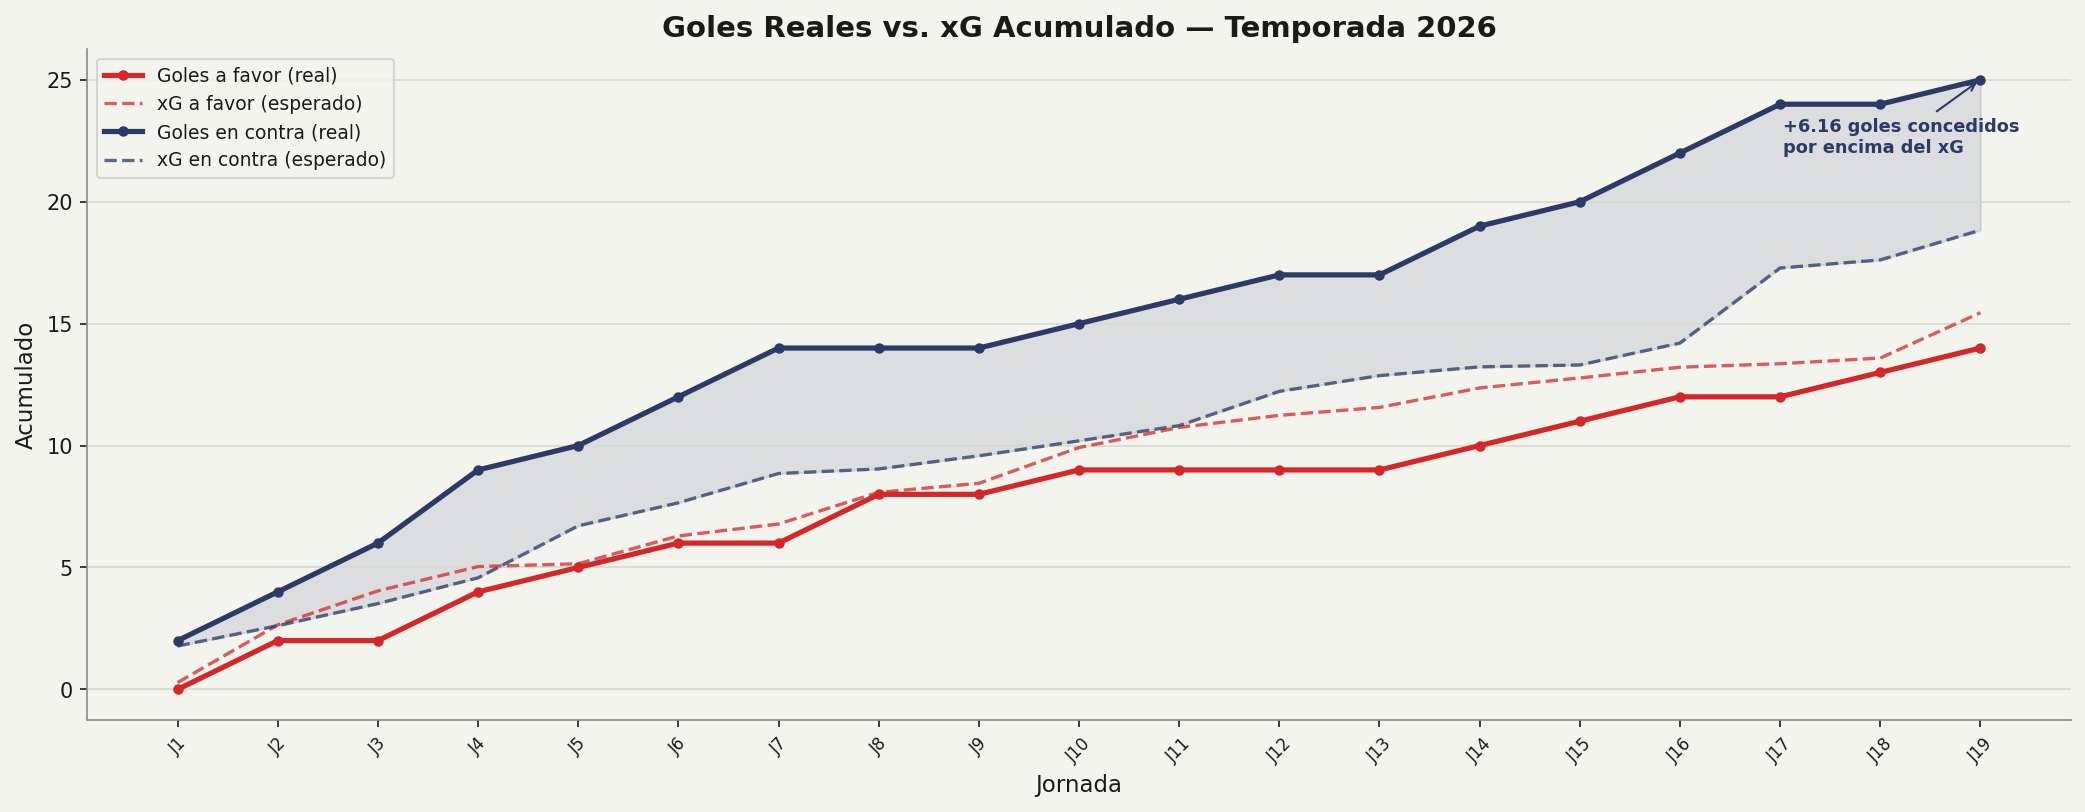
\includegraphics[width=0.98\textwidth]{evolution_xg_acumulado.png}}
  \caption{Goles reales frente a goles esperados (xG), acumulados fecha a fecha. La franja gris marca los $6.39$ goles que Chaco recibió por encima de lo que decía su xG en contra.}
  \label{fig:evolution_xg}
\end{figure}

% --- SECCIÓN 2: LOS TRES NUDOS CRÍTICOS ---
\section*{2. Los Tres Puntos Críticos}

\subsection*{Punto 1: no sostiene la ventaja}
Chaco se puso en ventaja de un gol en 3 partidos. En los 3 la perdió. En toda la temporada sumó apenas \mA{79 minutos} yendo arriba en el marcador, y en ese tramo recibió \mR{3 goles}.

La cadena de Markov lo confirma. Desde el empate, el equipo cae a desventaja el \mR{75\%} de las veces y se pone en ventaja solo el 20\%. Y cada vez que llegó a la ventaja, el \mR{100\%} de las veces volvió al empate. Nunca estiró la diferencia a dos goles estando arriba.

\subsection*{Punto 2: el arranque del complemento}
Entre el minuto 45 y el 60, Chaco recibió \mR{8 goles} y no marcó ninguno. Ahí cae el \mR{34.8\%} de todos los goles que le hicieron en el año. El patrón se repite fecha a fecha, no es un partido puntual.

El contraste llega enseguida: entre el 60 y el 75 el equipo marcó 4 goles y recibió 1. Es su mejor cuarto de hora. La caída, entonces, se concentra en los primeros minutos después del descanso. Los cambios y las piernas frescas suelen venir muy bien en estos minutos.

\subsection*{Punto 3: un ataque predecible}
Los remates de Chaco salen casi siempre del mismo lugar. Para medirlo usamos la entropía espacial: cuanto más alto es el valor, más repartidos están los tiros por toda la cancha; cuanto más bajo, más fácil es anticipar desde dónde ataca el equipo. Chaco registra \mA{1.655 sobre 4.644 bits}, apenas el 35.6\% del máximo posible. En términos simples: el ataque no está variando mucho sus zonas de finalización. El \mA{65\%} de los tiros nace de un solo sector, el centro del área. Si un rival cierra bien esa zona, apaga buena parte de la generación.

El circuito pasa por dos jugadores. Pacheco toca 468 balones en el último tercio y acumula \mA{130} en el área rival, casi el triple que el segundo, Enriquez, con 53. Marinucci juega el 54.5\% de sus toques en campo contrario. Desde el resto de las posiciones llega poco al frente.

% --- GRÁFICO 3: entropía espacial del ataque ---
\begin{figure}[htbp]
  \centering
  \fbox{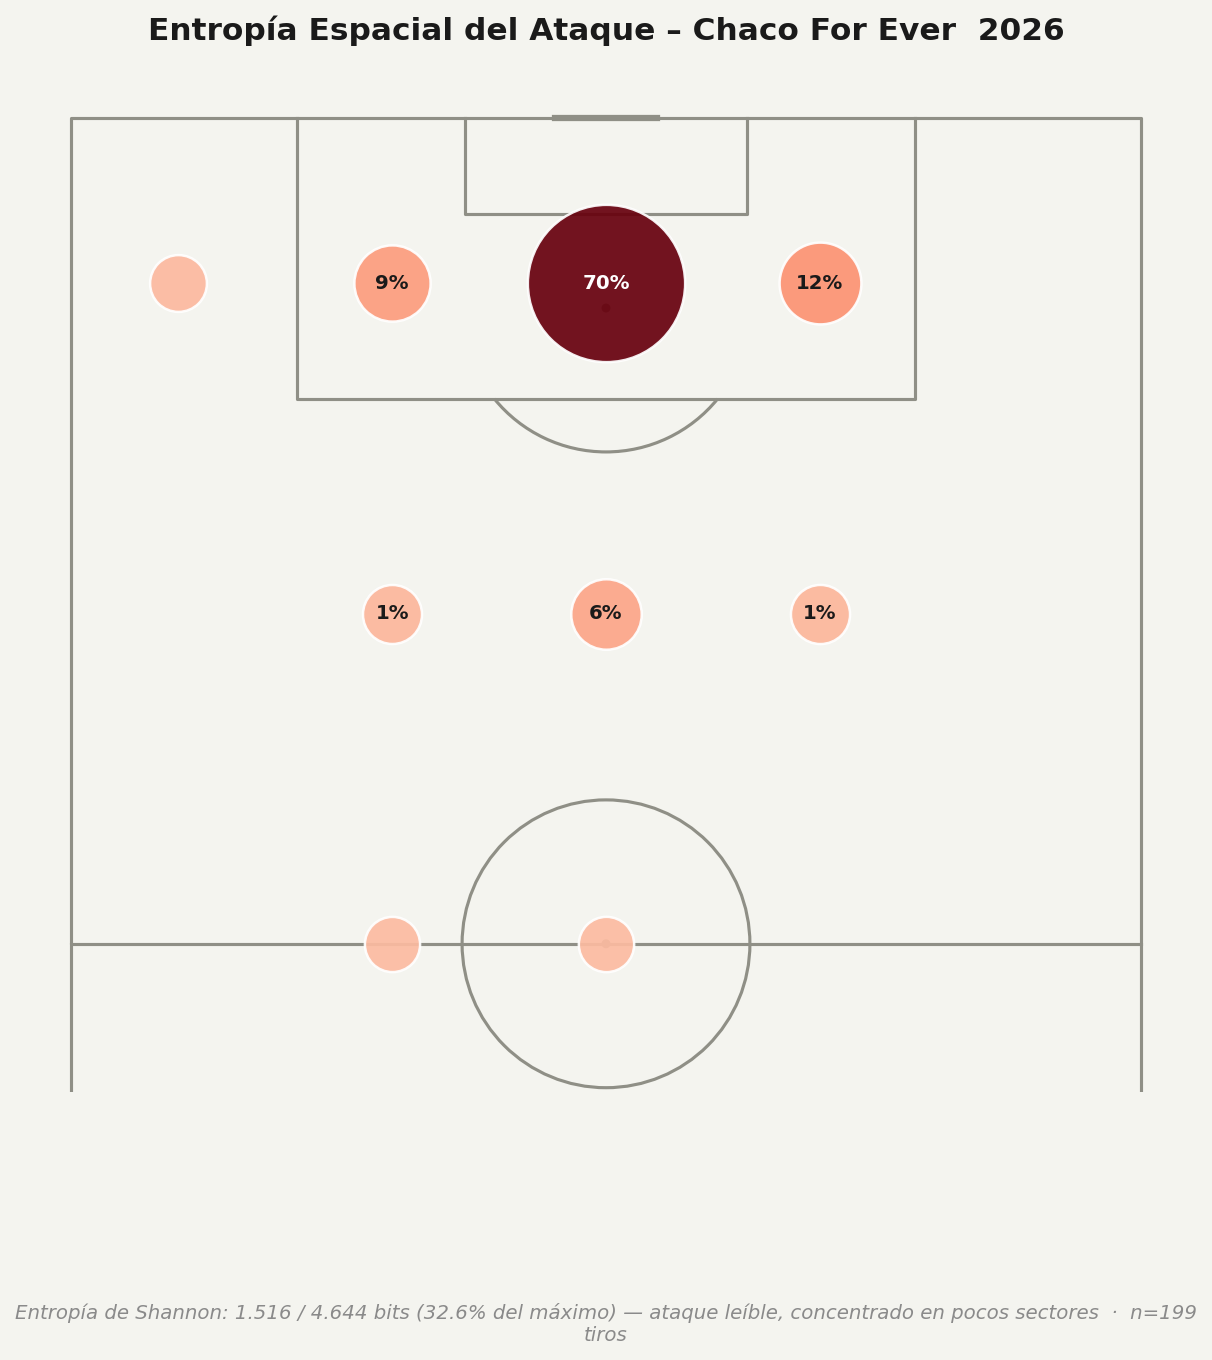
\includegraphics[width=1\textwidth]{entropia_tiros.png}}
  \caption{Origen de los disparos por sector de la cancha. El tamaño y color de cada burbuja marcan el porcentaje de tiros que salen de esa zona. El 65\% concentrado en el centro del área muestra un ataque leíble.}
  \label{fig:entropia}
\end{figure}

% --- GRÁFICO 2: goles por ventana horaria ---
\begin{figure}[htbp]
  \centering
  \fbox{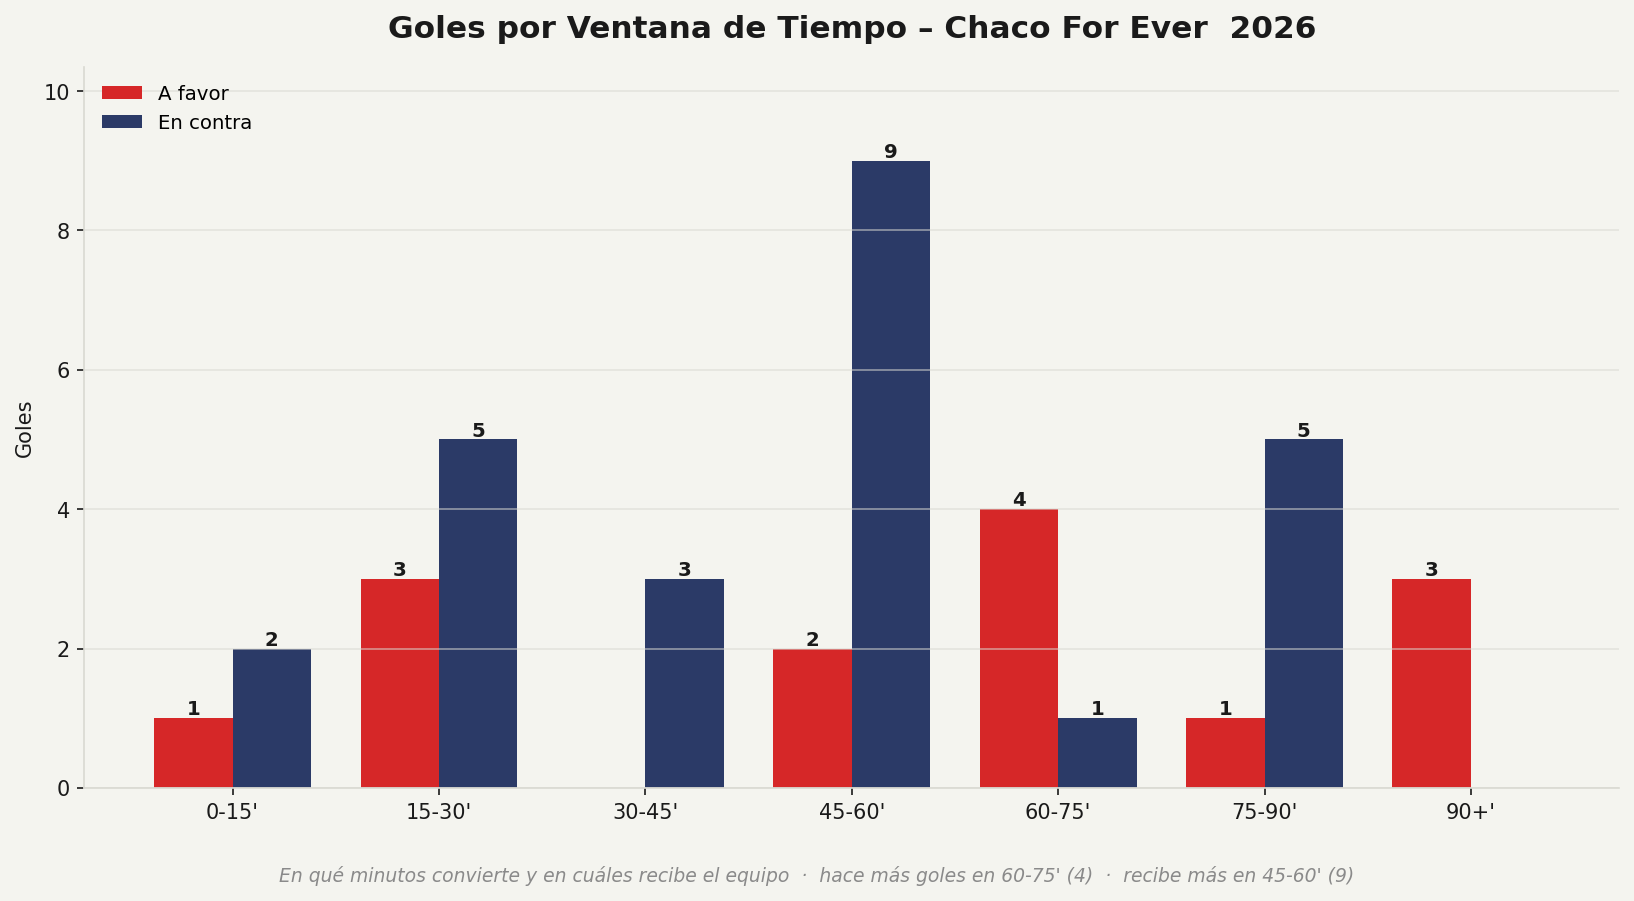
\includegraphics[width=0.98\textwidth]{goles_por_ventana_tiempo.png}}
  \caption{Goles a favor y en contra por ventana de 15 minutos. El pico rojo del 45 al 60 y el pico propio del 60 al 75 resumen el nudo 2.}
  \label{fig:ventanas_tiempo}
\end{figure}

% --- SECCIÓN 3: DE DÓNDE SALEN LOS GOLES ---
\section*{3. De Dónde Salen los Goles}

De los 13 goles de Chaco, 10 llegaron en juego abierto y \mA{3 de penal}. De córner, tiro libre, lateral o cualquier pelota parada: \mR{cero}. El equipo no convirtió un solo gol de balón detenido en 18 fechas. Casi un cuarto de sus goles depende de un penal.

En contra ocurre lo opuesto. De los 24 goles recibidos, 4 fueron de córner, y sumando tiro libre, lateral y pelota parada el total de balón parado llega a \mR{6 goles}. El equipo sufre en el área propia lo mismo que no aprovecha en la rival.

La creación también es escasa y está repartida. El máximo asistidor de la temporada, Melgarejo, tiene \mA{2 asistencias}. Nadie llegó a 3. Los 13 goles se repartieron entre 7 goleadores distintos, pero sin una sociedad que se repita: Pacheco y Marinucci, los dos que más patean, no se asistieron nunca entre sí.

% --- GRÁFICO 4: amenaza por tipo de jugada ---
\begin{figure}[htbp]
  \centering
  \fbox{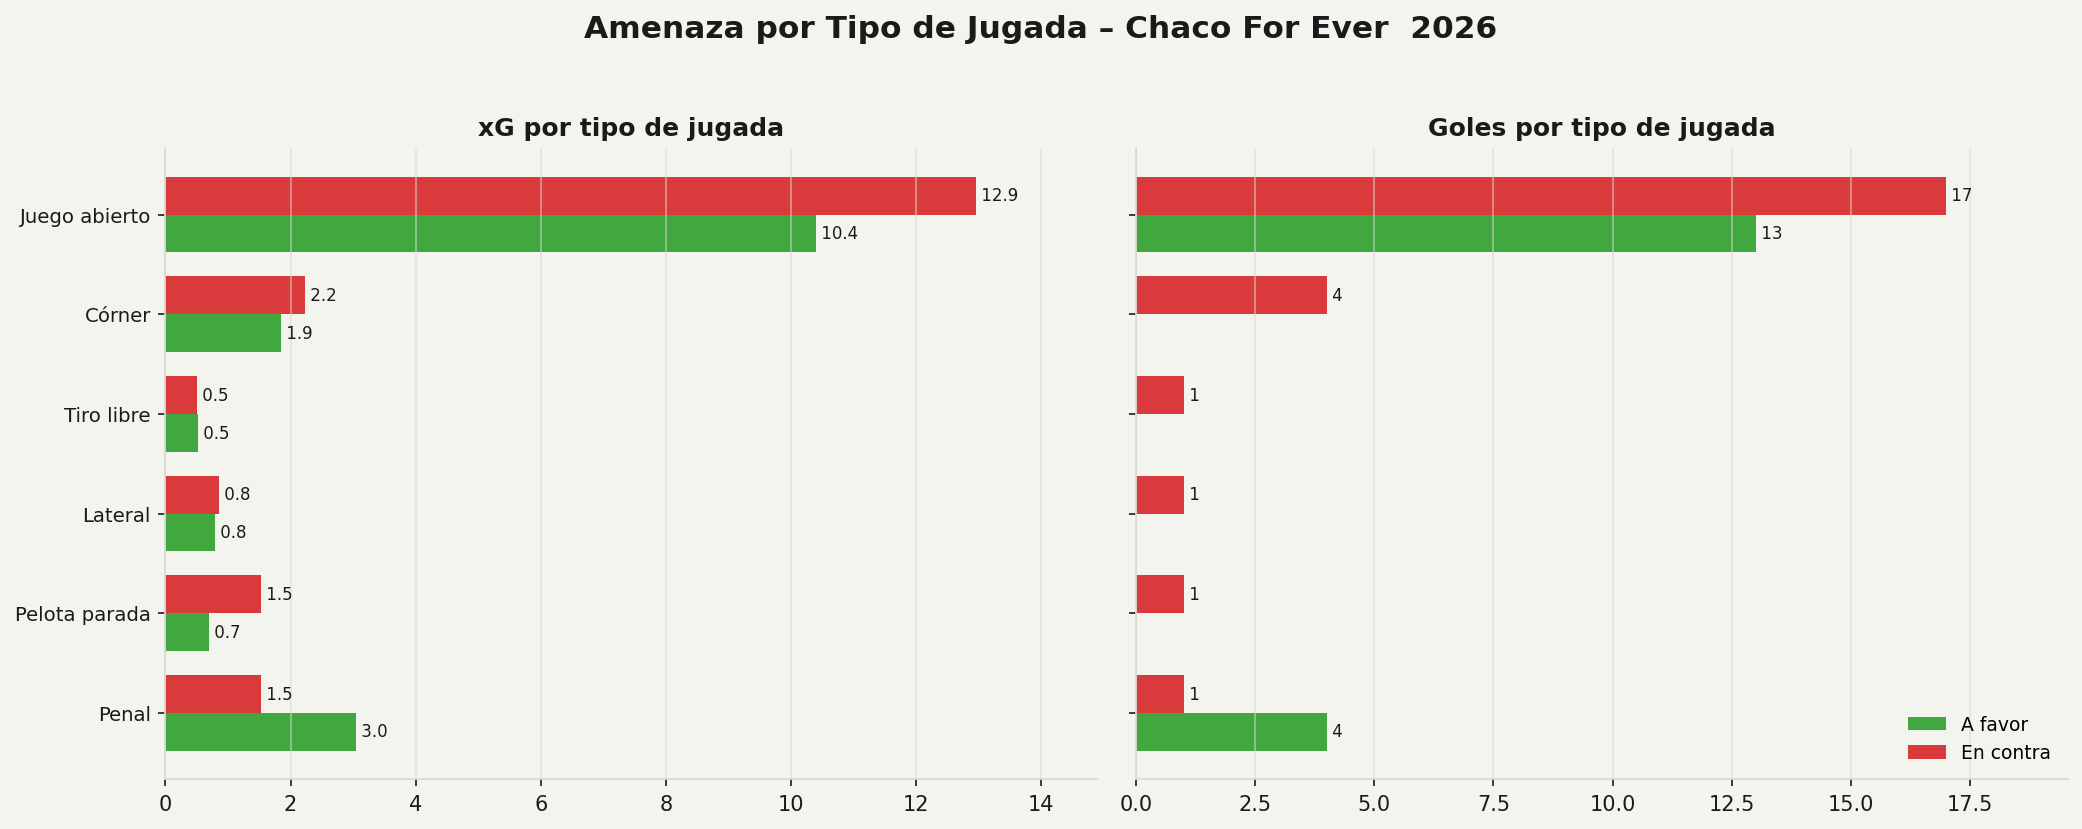
\includegraphics[width=0.98\textwidth]{amenaza_por_jugada.png}}
  \caption{xG y goles a favor y en contra según el tipo de jugada. A la derecha se ve la columna verde vacía en córner, tiro libre, lateral y pelota parada: Chaco no marcó de ninguna de esas situaciones.}
  \label{fig:amenaza}
\end{figure}

% --- SECCIÓN 4: INDIVIDUALES Y DISCIPLINA ---
\section*{4. Individuales y Disciplina}

\subsection*{Goleadores}
Marinucci lleva \mG{4 goles} con $2.47$ de xG. Convierte por encima de lo que generan sus situaciones. Pacheco suma 3 goles con $2.93$ de xG, justo en línea con lo que le llega. Entre los dos hacen 7 de los 13 goles del equipo.

\subsection*{Tarjetas}
Tres titulares están cerca de la suspensión:
\begin{itemize}
  \item \textbf{L. Pruzzo:} \mR{7 amarillas y 1 roja} en 13 partidos.
  \item \textbf{D. Valdez:} 5 amarillas y 1 roja. Es además el jugador con más peso en la red de pases, así que su ausencia le corta la salida al equipo.
  \item \textbf{B. Nievas:} 5 amarillas.
\end{itemize}

\vspace{1mm}
\hrule
\vspace{1mm}

\end{document}